\documentclass[preprint]{acm_proc_article-sp}
\usepackage{url}
\usepackage{graphicx,subfigure}
\usepackage{xspace}

\newcommand{\ie}{{\em i.e.,}~}
\newcommand{\eg}{{\em e.g.,}~}
\newcommand{\HadoopBM}{HadoopBinMem\xspace}

\newenvironment{denseitemize}{
\begin{itemize}[topsep=2pt, partopsep=0pt, leftmargin=1.5em]
  \setlength{\itemsep}{4pt}
  \setlength{\parskip}{0pt}
  \setlength{\parsep}{0pt}
}{\end{itemize}}

\begin{document}

\title{Shark: In-memory Interactive Analytics on Massive Datasets}

\numberofauthors{5}
\author{
Cliff Engle,
Antonio Lupher,
Reynold Xin,
Matei Zaharia,
Michael Franklin,
Ion Stoica\\\\
AMPLab, UC Berkeley\\
\texttt{\{cengle, alupher, rxin, matei, franklin\}@cs.berkeley.edu}
}

\maketitle
\begin{abstract}
This paper presents Shark.
\end{abstract}

% A category with the (minimum) three required fields
\category{H.4}{Information Systems Applications}{Miscellaneous}
%A category including the fourth, optional field follows...
\category{D.2.8}{Software Engineering}{Metrics}[complexity measures, performance measures]

\terms{Theory}

\keywords{databases, interactive queries, }


%%%%%%%%%%%%%%%%%%%%%%%%%%%%%%%%%%%%%%%%%%%%%%%%%%%%%%%%%%%%%%%%%%%%%%%%%%%%%%%
%%%%%%%%%%%%%%%%%%%%%%%%%%%%%%%%%%%%%%%%%%%%%%%%%%%%%%%%%%%%%%%%%%%%%%%%%%%%%%%
%%%%%%%%%%%%%%%%%%%%%%%%%%%%%%%%%%%%%%%%%%%%%%%%%%%%%%%%%%%%%%%%%%%%%%%%%%%%%%%

\section{Introduction}

Thanks to their flexibility, more and more structured and unstructured data are being stored in distributed file systems like HDFS. Apache Hive is a data warehousing infrastructure built on top of the Hadoop software stack. It provides an SQL-like declarative query language, HiveQL, which gets compiled into lower level operators that are executed in a sequence of MapReduce programs. 

Although Hive was designed to be a data warehousing solution, based on our discussions with many Hive users, a large percentage of Hive queries are ad-hoc, exploratory in nature and issued from the Hive console rather than programmatically generated for traditional data warehousing reports. Take Facebook for example. Their Hadoop clusters are dominated by jobs generated from Hive \cite{hive} queries. Even though the queries are intended to be exploratory, median map and reduce job duration is 84s \cite{delay-scheduling}. Note that typical query duration would be a multiple of this number since a query consists of multiple stages of map and reduce jobs. There is a tremendous difference in interactivity between queries that run in seconds versus minutes or hours.

There is a clear need for interactive query systems for large data sets and the industry is exploring solutions. A prime example is Google's Dremel \cite{dremel}, which achieves interactivity through a combination of employing projection indexes (columnar store) and parallelizing query execution across thousands of machines to improve disk throughput. Most organizations, however, cannot afford to have thousands of machines. We argue the only and a better way to achieve interactivity is by caching data in memory.

In \cite{memento-hotos}, Ananthanarayanan et al analyzed the access patterns in the Hive warehouses at Facebook. They discovered that, surprisingly, for vast majority (96\%) of jobs, the entire inputs can fit into a fraction of the cluster's total memory. This finding might be counterintuitive for a petabyte scale warehouse. But imagine in a warehouse where the fact table contains petabytes of data, it is unlikely we need the entire fact table to answer all queries. Queries usually focus on a particular window, \eg http logs from last month, touching only the dimension tables and small portion of the fact table. It is thus plausible to fit the working set into a cluster's memory.

- on the other hand, machine learning / data scientists appreciate the ability to use sql to explore and manipulate data before running their machine learning algorithms.

- people have been proposing machine learning algorithm implementations in sql in traditional relational databases \cite{madlib}.

- there is a need for running machine learning in hive.

In the remainder of this demonstration proposal, we outline Shark's system design, and explain briefly how it achieves low-latency and enables interactivity. Finally, we describe the 


%%%%%%%%%%%%%%%%%%%%%%%%%%%%%%%%%%%%%%%%%%%%%%%%%%%%%%%%%%%%%%%%%%%%%%%%%%%%%%%
%%%%%%%%%%%%%%%%%%%%%%%%%%%%%%%%%%%%%%%%%%%%%%%%%%%%%%%%%%%%%%%%%%%%%%%%%%%%%%%
%%%%%%%%%%%%%%%%%%%%%%%%%%%%%%%%%%%%%%%%%%%%%%%%%%%%%%%%%%%%%%%%%%%%%%%%%%%%%%%
\section{Resilient Distributed Datasets}
In this section, we explain reasons why we choose to implement Shark on top of Spark. We first give a brief overview of Spark and Resilient Distributed Datasets (RDDs). Due to space constraints, we refer readers to \cite{spark-tr} for more details.

RDD is a fault-tolerant clustering computing abstraction that suits particularly well for low-latency interactive applications. Formally, an RDD is an immutable, partitioned collection of records that can only be created through deterministic \emph{transformations} on either data in stable storage (\eg files in HDFS) or other RDDs. Examples of transformations include \emph{map}, \emph{filter}, \emph{reduce}, and \emph{join}. Note that RDDs do not need to be materialized at all times, as they can be reconstructed based on lineage information. Users can control two aspects of RDDs: \emph{persistence} and \emph{partitioning}. Using the persistence API, users can indicate which RDDs they will reuse and choose a storage strategy for them (\eg caching them in memory). This is particularly useful in cache investment as the higher level program can choose to materialize certain RDDs in memory and reuse them later. For workloads that require going through data multiple times, such as interactive queries and iterative machine learning queries, Spark's persistence feature is very attractive. They can also ask that an RDD's elements be partitioned across machines based on key in each record. This is useful for placement optimizations, such as ensuring that two datasets that will be joined together are hash-partitioned in the same way.

Spark provides the RDD abstraction through a language-integrated API in Scala, a statically typed functional programming language for the Java VM. Each RDD dataset is represented as a Scala object, while the transformations are invoked using methods on those objects. To use Spark, developers write a driver program that connects to a cluster of workers. The driver defines one or more RDDs and invokes actions on them. The workers are long-lived processes that can store dataset partitions in memory across operations.

As an example, the following program implements k-means clustering, a common cluster analysis algorithm that partitions n points into k clusters represented by the centroids. The algorithm is iterative: the k centroids are initialized randomly, and on each iteration, the points are assigned to the cluster with the nearest centroids, and then the centroids are recalculated based on the points in the clusters. {\small
\begin{verbatim}
def kmeans(points: RDD[Point], k: Int) = {
  // Initialize the centroids.
  clusters = new HashMap[Int, Point]
  for (i <- 0 until k) centroids(i) = Point.random()

  for (i <- 1 until 10) {
    // Assign points to centroids and update centroids.
    clusters = points.groupBy(closestCentroid)
      .map{ 
         (id, points) => (id, points.sum / points.size)
      }.collectMap()
  }
}
\end{verbatim}
}

%%%%%%%%%%%%%%%%%%%%%%%%%%%%%%%%%%%%%%%%%%%%%%%%%%%%%%%%%%%%%%%%%%%%%%%%%%%%%%%
%%%%%%%%%%%%%%%%%%%%%%%%%%%%%%%%%%%%%%%%%%%%%%%%%%%%%%%%%%%%%%%%%%%%%%%%%%%%%%%
%%%%%%%%%%%%%%%%%%%%%%%%%%%%%%%%%%%%%%%%%%%%%%%%%%%%%%%%%%%%%%%%%%%%%%%%%%%%%%%
\section{Shark}
Shark is designed to be entirely hot-swappable with Hive. Anyone can put Shark up and running in an existing Hive warehouse without any modification to existing data. Existing queries will return the same set of results, albeit much faster.

Shark's overall architecture is quite similar to that of Apache Hive in order to provide maximum interoperability. Data are stored physically in the underlying distributed file system HDFS. The Hive metastore is used as is in Shark and tracks the metadata and statistics about tables, much like the system catalog found in traditional relational databases. 

From a higher level, Shark's query execution is very similar to Hive as well as traditional relational databases. In fact, Shark uses Hive as a third-party Java library for query parsing and logical plan generation. The main difference is in the physical plan execution.

Given a HiveQL query, the Hive query compiler is used to parse the query and generate an abstract syntax tree. The tree is then turned into the logical plan, a tree of logical operators (e.g. Table Scan, Filter, Select, Join and Group-By) and basic logical optimization such as predicate push downs are applied. Up until this point, Shark and Hive follow identical process. In Hive, this operator tree would be converted into a physical plan that consists of subtrees for separate map reduce tasks to have tuples streamed through them. In Shark, this operator tree is converted into Shark operators that perform transformations on Spark RDDs. An iterator traverses the operator tree and produces an immutable RDD for each operator on the tree. This RDD is lazily evaluated when the the execution engine finishes processing the operators and query results are returned. 

Much of the common structure of Hive operators is retained in order to ensure interoperability with HiveQL. We have currently implemented support for all of the essential Hive operators. We reuse all of Hive's data model and type system, in addition to supporting Hive's user-defined functions, user-defined aggregate functions, custom types, and custom serialization/deserialization methods. Shark also operates on the same metastore as Hive and is entirely hot-swappable with Hive.

\begin{figure}[h*]
	\centering
	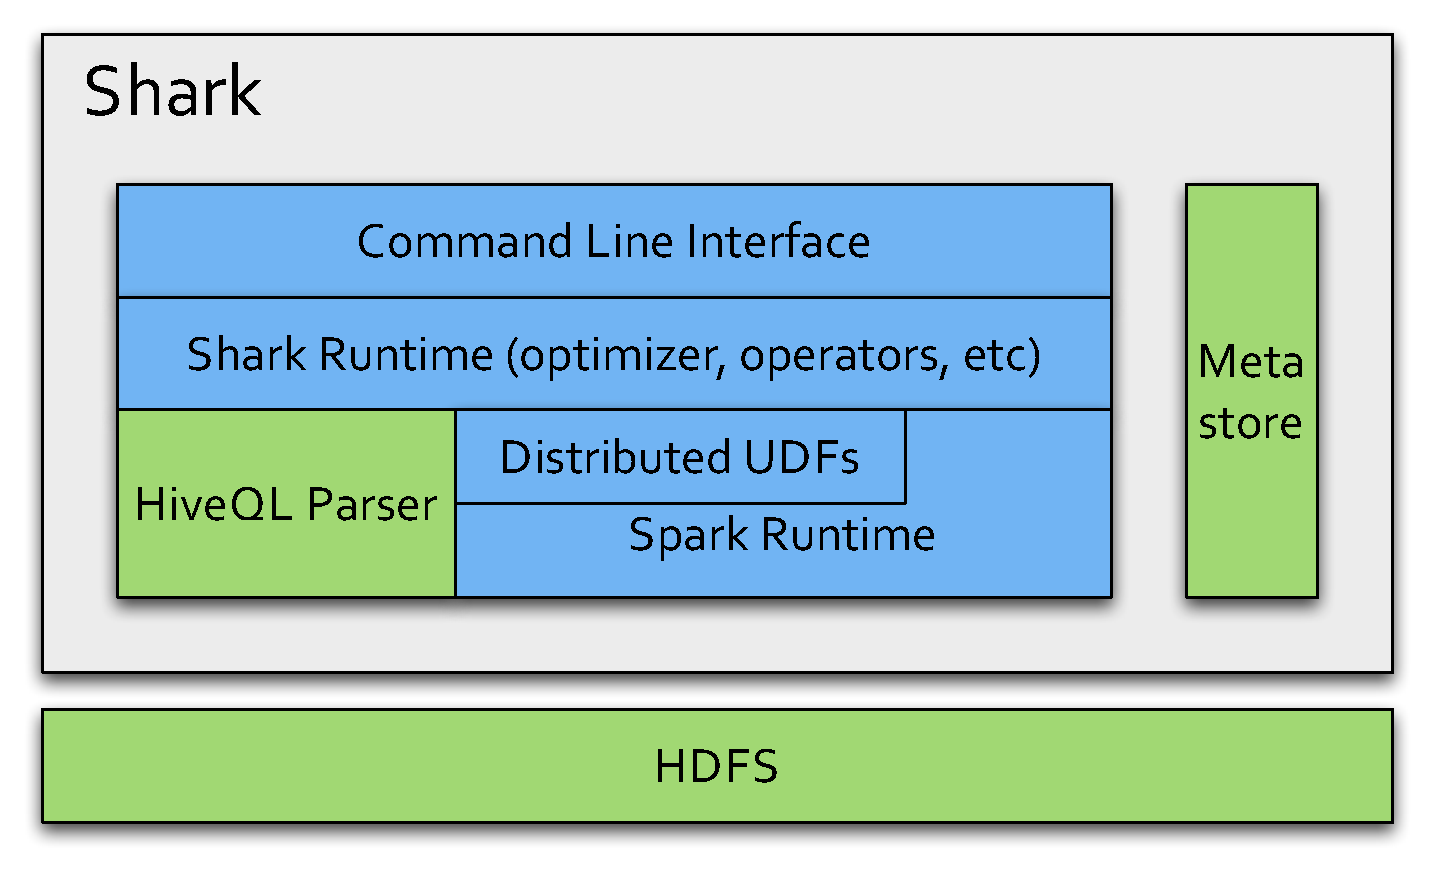
\includegraphics[width=\linewidth]{files/architecture.pdf}
	\caption{Shark Architecture}
	\label{fig:arch}
\end{figure}

A major advantage Shark has over Hive is the inter-query caching of data. The Spark framework provides a simple mechanism to cache RDD in memory across clusters and recompute RDDs in the event of failures. In Shark, each operator subtree's result is cached automatically, and a signature is computed for the subtree. This signature, along with a timestamp of the original file's last modified time in HDFS, is stored in a table in the metastore. Signatures are computed for subsequent query subtrees and are compared to those in the table and, in case of a match, the in-memory RDD is utilized. Cache invalidation is handled by checking the timestamp of the last modification of the HDFS data to the timestamp stored in our mapping. We have implemented a variety of simple cache replacement algorithms such as LFU, LRU and are currently exploring more sophisticated algorithms that perform cost-benefit analysis.

Another advantage of Shark is the ease of combining machine learning algorithms with SQL over data, which is done through table-valued user-defined functions. Shark provides a simple API for these UDFs, which accept a \emph{Table} object as input, and emit a \emph{Table} object for output. We have already implemented a number of basic machine learning algorithms, e.g. linear regression, logistics regression, k-means. In most cases, the user only need to implement a UDF that transforms the input \emph{Table} object into the desired input data type for the selected algorithm and transform the output from the algorithm into a separate \emph{Table} object. For example, in the case of k-means, selecting the desired columns to generate the RDD of points for input, and adding an extra column for cluster ID for output. Short UDFs can also be embedded inline in queries in Shark's interactive mode, in part thanks to the conciseness of anonymous functions in Scala.


%%%%%%%%%%%%%%%%%%%%%%%%%%%%%%%%%%%%%%%%%%%%%%%%%%%%%%%%%%%%%%%%%%%%%%%%%%%%%%%
%%%%%%%%%%%%%%%%%%%%%%%%%%%%%%%%%%%%%%%%%%%%%%%%%%%%%%%%%%%%%%%%%%%%%%%%%%%%%%%
%%%%%%%%%%%%%%%%%%%%%%%%%%%%%%%%%%%%%%%%%%%%%%%%%%%%%%%%%%%%%%%%%%%%%%%%%%%%%%%
\section{Performance Gains}

\subsection{Conviva Warehouse}
Conviva Inc, a video distribution company, used Spark to accelerate a number of data analytics reports that previously ran over Hive. For example, one report ran as a series of Hive queries that computed various statistics for a customer. These queries all worked on the same subset of the data (records matching a customer-provided predicate), but performed aggregations (averages, percentiles, and {\small\tt COUNT DISTINCT}) over different grouping fields, requiring separate MapReduce jobs. By implementing the queries in Spark and loading the data shared across them into an RDD, the company was able to speed up the report by $40\times$. A report on 200 GB of compressed data that took 20 hours on a Hadoop cluster now runs in 30 minutes using only two Spark machines and 96 GB RAM. The speedup comes from a combination of keeping the columns of interest in memory and avoiding repeated decompression and filtering of the same data files.

Conviva is now running approximately 30\% of its analytics reports on Spark instead of Hive, but this required manual porting of SQL queries to Spark. With Shark, they expect to be able to automatically port the other reports as well.

In addition, a number of users in Conviva use Hive interactively for debugging (e.g., finding commonalities between users who experienced low video quality to identify misconfigurations and software bugs). Like the analytics reports, these queries repeatedly access and refine the same dataset, so running them over Shark would greatly reduce debug cycles.

\subsection{Iterative Machine Learning}

Many machine learning algorithms are iterative in nature because they run iterative optimization procedures, such as gradient descent, to optimize an objective function. These algorithms can be sped up substantially using Shark if their working set fits into RAM across a cluster. Furthermore, these algorithms often employ bulk operations like maps and sums, making them easy to express with RDDs in UDFs.

We implemented two iterative machine learning algorithms, logistic
regression and k-means, to compare the performance of the
following system setup:\vspace{-10pt}\begin{itemize}
  \setlength{\itemsep}{4pt}
  \setlength{\parskip}{0pt}
  \setlength{\parsep}{0pt}
  \item Hadoop: The Hadoop 0.20.2 stable release.
  \item \HadoopBM: A Hadoop deployment that converts the input
  data into a low-overhead binary format in the first iteration to eliminate
  text parsing in later ones, and stores it in an in-memory HDFS instance.
  \item Shark: Algorithms implemented in Spark and invoked using table-valued user-defined functions.
\end{itemize}

\begin{figure}[!t]
	\centering
	\subfigure[][Logistic Regression]{%
		\label{fig:lr-later-absol}%
		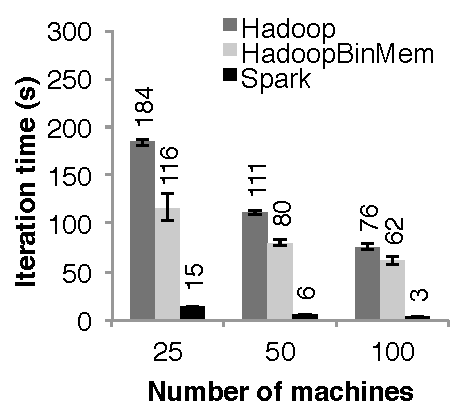
\includegraphics[scale=0.52]{files/lr-later-absol-THIN}%
	}%
	%\hspace{3pt}
	\subfigure[][K-Means]{%
		\label{fig:km-later-absol}%
		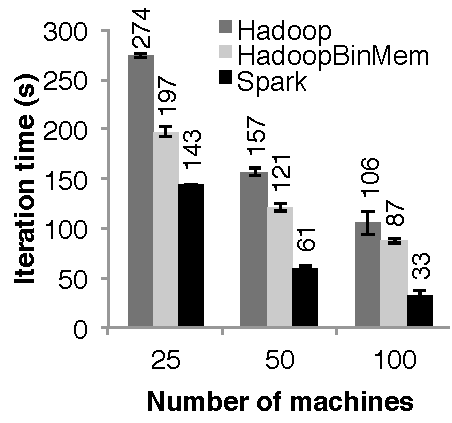
\includegraphics[scale=0.52]{files/km-later-absol-THIN}%
	}%
	%\hspace{8pt}	
	\caption[LR and KM performance]{Runtime comparison for Hadoop and Spark}%
	\label{fig:tstm}
\end{figure}

We ran both algorithms for 10 iterations on 100 GB datasets using 25--100 machines. The key difference between the two algorithms is the amount of computation they perform per byte of data. The
iteration time of k-means is dominated by computation, while
logistic regression is less compute-intensive and thus more sensitive
to time spent in deserialization and I/O.

Since typical learning algorithms need tens of iterations to converge,
we report times for the first iteration and subsequent iterations separately.
We find that sharing data via RDDs greatly speeds up future iterations. Note that by the time the user runs the machine learning algorithms in Shark, the working set are likely to be already in memory through the SQL manipulations.

Figure~\ref{fig:tstm} shows how these scaled with cluster size. For logistic regression, Shark was $25.3\times$ and $20.7\times$ faster than Hadoop and \HadoopBM respectively on 100 machines. For the more compute-intensive k-means application, Shark still achieved speedup of $1.9\times$ to $3.2\times$.


%%%%%%%%%%%%%%%%%%%%%%%%%%%%%%%%%%%%%%%%%%%%%%%%%%%%%%%%%%%%%%%%%%%%%%%%%%%%%%%
%%%%%%%%%%%%%%%%%%%%%%%%%%%%%%%%%%%%%%%%%%%%%%%%%%%%%%%%%%%%%%%%%%%%%%%%%%%%%%%
%%%%%%%%%%%%%%%%%%%%%%%%%%%%%%%%%%%%%%%%%%%%%%%%%%%%%%%%%%%%%%%%%%%%%%%%%%%%%%%
\section{Demonstration Details}

In this demonstration, we present an end-to-end implementation of Shark and emphasize its interactive nature. Demonstration attendees will assume the role of a data journalist that wants to analyze an one-terabyte collection of tweets. 

The demonstration exhibits three main components:

\textbf{Data Set}: We will have a HDFS cluster on Amazon EC2 hosting one terabyte of tweets, collected using the Twitter streaming API prior to the conference.

\textbf{Shark and Hive Clusters}: During the demo, we will have a 100-node Shark cluster and an equal-sized Apache Hive cluster running on EC2 for side-by-side comparison.

\textbf{Web Console}: Since it is hard to capture the internals of query processing given only the query and the output, we have implemented a web console that illustrates the query plan, the caching of RDDs for multi-query optimization, and status of the distributed Spark nodes. In addition, to demonstrate Shark's fault-tolerance feature, we will arbitrarily submit kill signals to Spark nodes from the web console.

SIGMOD attendees will be able to run queries outlined in predefined story line as well as ad-hoc exploration of the data set through the command-line interface. They will be able to compare the two systems, noticing the stark contrast in interactivity between Shark and Hive. Next we describe in detail the demo story line.

\subsection{Story Line}

As stated earlier, demo attendees will assume the role of a data journalist. They first generate a histogram of the number of tweets and realize there is a spike in early October. Since Twitter activities usually correlate with events, they would like to gain insights about such events by understanding the causes for the spike. To do so, they drill down to focus on the particular two weeks, and run clustering algorithms on the tweets. They then realize there are three large clusters, implying three concurrent events from which the tweets come: the decease of Steve Jobs, the decease of Dennis Ritchie, and the Occupy Wall Street movement.

Suppose then they decide to write a piece about the movement, and want to find out the public's sentiment towards this movement. Since it is unlikely for the world to have one agreeing view on this particular issue, they would like to break the sentiment down by country and state. He achieves this by doing a group by on geographical locations and running the sentiment analysis algorithm, which is simply a user-defined aggregate function in Shark.

%%%%%%%%%%%%%%%%%%%%%%%%%%%%%%%%%%%%%%%%%%%%%%%%%%%%%%%%%%%%%%%%%%%%%%%%%%%%%%%
%%%%%%%%%%%%%%%%%%%%%%%%%%%%%%%%%%%%%%%%%%%%%%%%%%%%%%%%%%%%%%%%%%%%%%%%%%%%%%%
%%%%%%%%%%%%%%%%%%%%%%%%%%%%%%%%%%%%%%%%%%%%%%%%%%%%%%%%%%%%%%%%%%%%%%%%%%%%%%%

\section{Acknowledgments}
This research is supported in part by gifts from Google, SAP, Amazon Web Services, Cloudera, Ericsson, Huawei, IBM, Intel, Mark Logic, Microsoft, NEC Labs, Network Appliance, Oracle, Splunk and VMWare and by DARPA (contract \#FA8650-11-C-7136).

\bibliographystyle{abbrv}
\bibliography{paper}

\balancecolumns
\end{document}
